\section{MPI}

Boilerplate: 
\begin{minted}[breaklines]{C}
#include "mpi.h"
int main(int argc, char** argv) {
    int size, rank;
    MPI_Init(&argc, &argv);
    MPI_Comm_size(MPI_COMM_WORLD, size);
    MPI_Comm_rank(MPI_COMM_WORLD, rank);
    if(rank == 0) { /*... */ } else { /* ... */ } // Root node check
    MPI_Finanlize();
    return 0;
}
\end{minted}

\subsection{Functions}

\begin{minted}[breaklines]{C}
MPI_Barrier(MPI_Comm comm);

int MPI_Send(void* buffer, int count, MPI_Datatype datatype, int dest, int tag, MPI_Comm comm);

int MPI_Recv(void* buffer, int count, MPI_Datatype datatype, int source, int tag, MPI_Comm comm, MPI_Status* status);

int MPI_Bcast(void* buffer, int count, MPI_Datatype t, int root, MPI_Comm comm);

int MPI_Scatter(void* sendbuf, int sendcount, MPI_Datatype sendtype, void* recvbuf, int recvcount, MPI_Datatype recvtype, int root, MPI_Comm comm);

int MPI_Gather(void* sendbuf, int sendcount, MPI_Datatype sendtype, void* recvbuf, int recvcount, MPI_Datatype recvtype, int root, MPI_Comm comm);

int MPI_Allgather( void* sendbuf, int sendcount, MPI_Datatype sendtype, void* recvbuf, int recvcount, MPI_Datatype recvtype, MPI_Comm comm);

int MPI_Alltoall( void *sendbuf, int sendcount, MPI_Datatype sendtype, void *recvbuf, int recvcount, MPI_Datatype recvtype, MPI_Comm comm);

int MPI_Reduce(void* sendbuf, void* recvbuf, int count, MPI_Datatype type, MPI_Op op, int root, MPI_Comm comm);
\end{minted}
\begin{center}
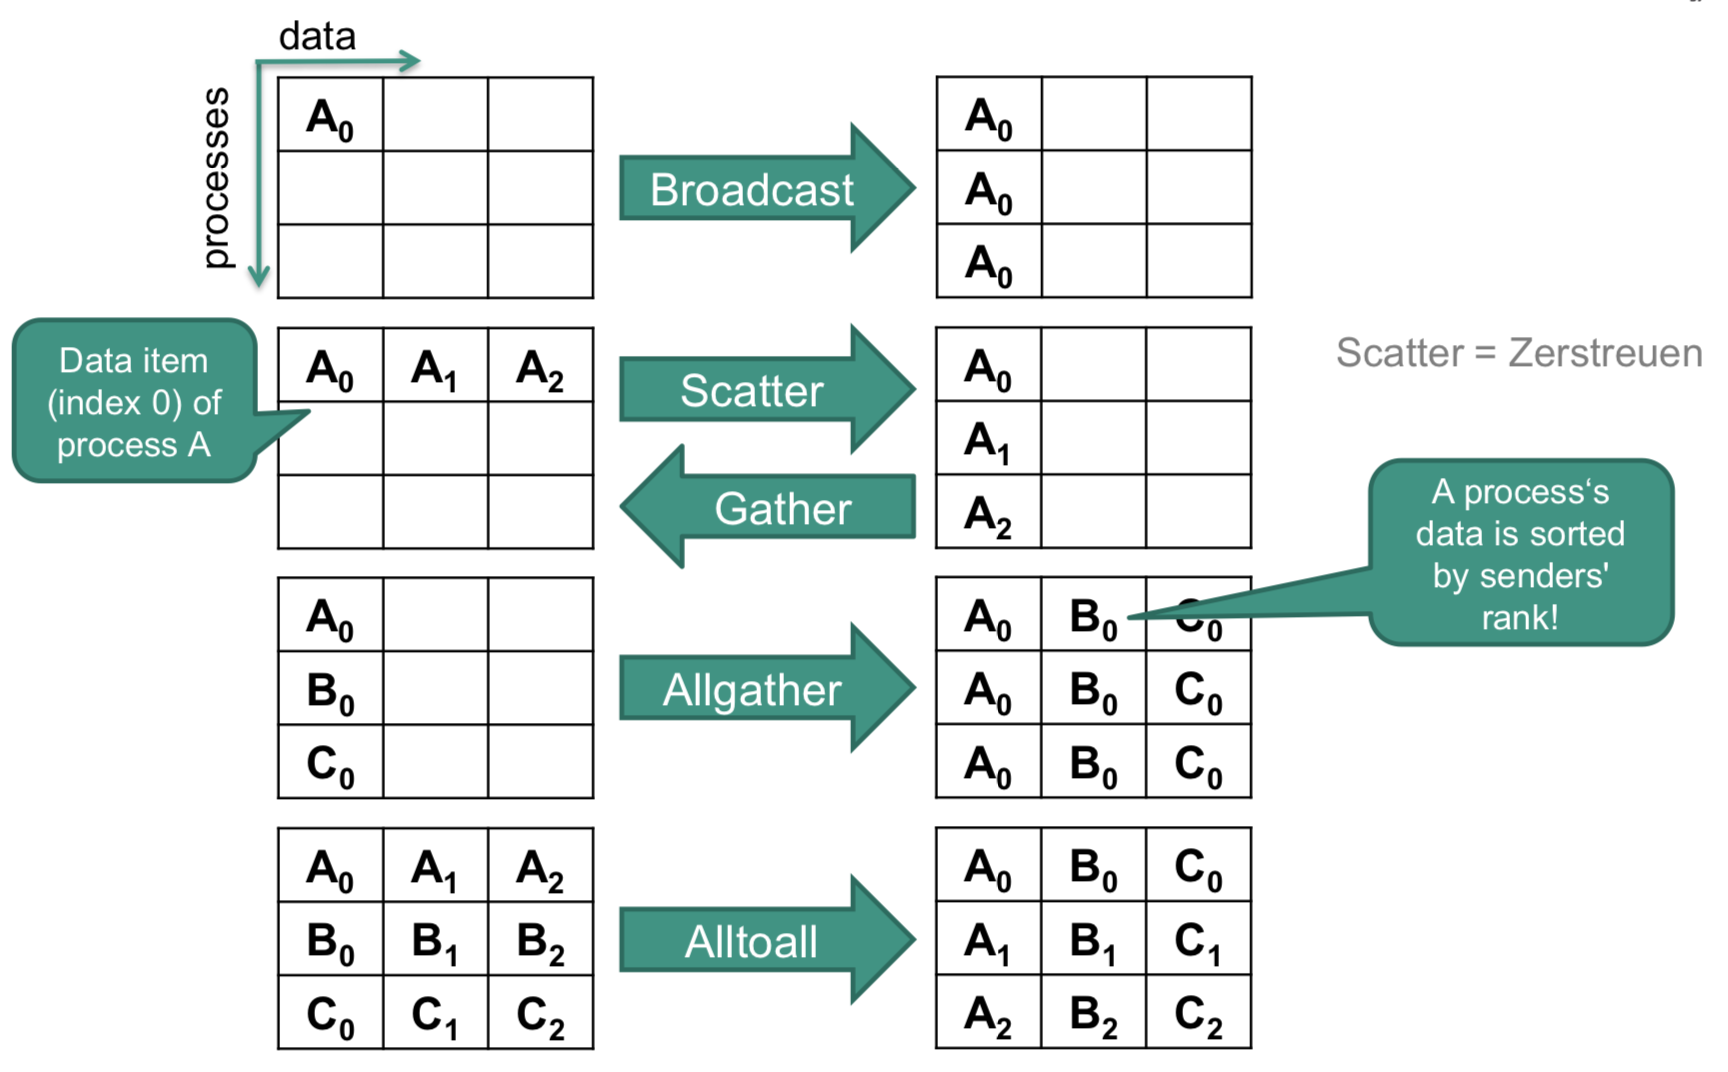
\includegraphics[width=\columnwidth]{images/MPI.png}
\end{center}
Example:
\begin{minted}[breaklines]{C}
if (myrank == 0) {
    strcpy(msg, "Hello student!");
    MPI_Send(msg, strlen(msg)+1, MPI_CHAR, 1, tag, MPI_COMM_WORLD);
} else {
    MPI_Recv(msg, 20, MPI_CHAR, 0, tag, MPI_COMM_WORLD, &status); 
    printf("received \"%s\"\n", msg);
}
\end{minted}
MPI-Datatypes: \texttt{MPI\_INT, MPI\_CHAR, MPI\_FLOAT,  MPI\_DOUBLE, ...}\\

\paragraph{Operations for \texttt{MPI\_Reduce}}
Mathematical Operations : \texttt{MPI\_MAX , MPI\_MIN , MPI\_SUM , MPI\_PROD} \\
Boolean Operations (logical and bitwise): \texttt{MPI\_LAND , MPI\_BAND , MPI\_LOR , MPI\_BOR, ...}\\

\subsection{Modes}

Blocking (default) vs. non-blocking\\

\textbf{Send-modes:}
\begin{enumerate}
	\item Synchronous: No buffer, synchronization (both sides wait for each other)
	\item Buffered:	Explicit buffering, no synchronization (no wait for each other)
	\item Ready: No buffer, no synchronization, matching receive must already be initiated
	\item Standard: May buffer or not, can be synchronous (implementation dependent)
\end{enumerate}




